% Gemini theme
% https://github.com/anishathalye/gemini

\documentclass[final]{beamer}

% ====================
% Packages
% ====================

\usepackage[T1]{fontenc}
\usepackage{lmodern}
\usepackage[size=custom,width=101.6,height=76.2,scale=1.0]{beamerposter}
\usetheme{gemini}
\usecolortheme{umn}
\usepackage{graphicx}
\usepackage{booktabs}
\usepackage{tikz}
\usepackage{pgfplots}
\pgfplotsset{compat=1.14}
\usepackage{anyfontsize}

% ====================
% Lengths
% ====================

% If you have N columns, choose \sepwidth and \colwidth such that
% (N+1)*\sepwidth + N*\colwidth = \paperwidth
\newlength{\sepwidth}
\newlength{\colwidth}
\setlength{\sepwidth}{0.025\paperwidth}
\setlength{\colwidth}{0.3\paperwidth}

\newcommand{\separatorcolumn}{\begin{column}{\sepwidth}\end{column}}

% ====================
% Title
% ====================

\title{Phase-Sense: Physics Guided AI}

\author{Joel Kuehne \and Alexis MacLean \and Cole Jaeger \and Hamza Rahmoune }

\institute[shortinst]{Department of Electrical and Computer Engineering, University of Minnesota Twin Cities}

% ====================
% Footer (optional)
% ====================

% \footercontent{
%   \href{https://www.example.com}{https://www.example.com} \hfill
%   ABC Conference 2025, New York --- XYZ-1234 \hfill
%   \href{mailto:alyssa.p.hacker@example.com}{alyssa.p.hacker@example.com}}
% (can be left out to remove footer)

% ====================
% Logo (optional)
% ====================

% use this to include logos on the left and/or right side of the header:
\logoleft{
\includegraphics[height=7cm]{M_gold.png}}
% \logoleft{\includegraphics[height=7cm]{logo2.pdf}}

% ====================
% Body
% ====================

\begin{document}

\begin{frame}[t]
\begin{columns}[t]
\separatorcolumn

\begin{column}{\colwidth}

  \begin{block}{Emergent Phenomena and Colloidal Aggregation}
    To cite Cambridge Dictionary, ``An emergent property of a complex system is one that does not belong to any part of that system on its own, but that happens as a result of parts of the system interacting''. This could be particles colliding in a fluid and sticking together forming clusters or it could be individual atoms joining together during crystal growth.

    Emergent phenomena are everywhere, and the analysis of emergent phenomena is useful in many fields. When trying to understand or analyze emergent phenomena, it is useful to have some measure of the relative progress of the phenomenon. In general, we call this measure of the relative progress of the event over time the ``emergence index''. A plot of the emergence index over time is therefore an ``emergence curve''.

    Researchers at the University of Pennsylvania use this framework in their analysis of the aggregation of asbestos particles in the paper ``Aggregation of Elongated Colloids in Water''~\cite{aggr}. Figure~\ref{fig:emergence} below shows some of the emergence curves that they gathered from timelapse microscope video. Note the three distinct phases of aggregation. In Phase I, aggregation has not yet started. There is a distinct onset time between Phase I and Phase II, where aggregation takes off. By Phase III, the aggregation has completed and the emergence curve levels off.

    \begin{figure}[h]
      \centering
      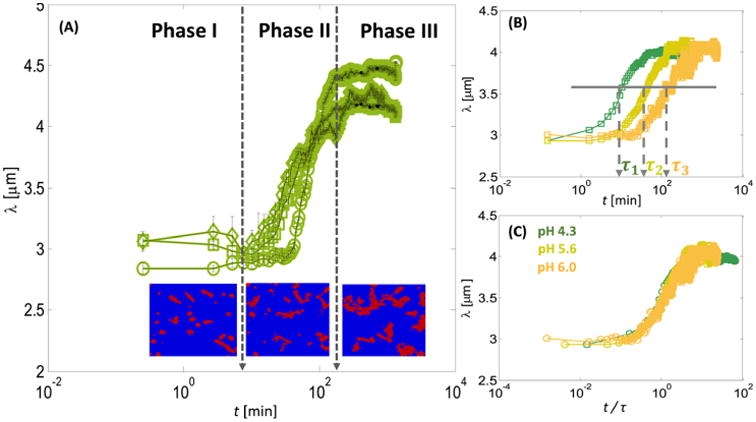
\includegraphics[width=0.9\textwidth]{emergence.jpg}
      \caption{Emergence curves for the aggregation of asbestos particles~\cite{aggr}.}
      \label{fig:emergence}
    \end{figure}
  \end{block}

  \begin{block}{Neural Networks for Emergence Analysis}
    Analysis of emergent phenomena can be difficult. Classical computer vision techniques work well when particles can be easily distinguished and the emergence index can be calculated directly. This is not always the case. Low resolutions, small particle sizes, and lens aberrations can all complicate conventional analysis. Neural networks have proved to be quite effective in this regard~\cite{htt}, but require large, annotated datasets of microscope footage as training data.

    With our project, Phase-Sense, we hope to show that neural networks trained on physically-accurate, simulated footage can provide an improvement over classical computer vision techniques in the analysis of emergent phenomena in timelapse microcopy. Our project consists of three parts:

    \begin{enumerate}
      \item \textbf{PyTorch Neural Network} --- Analyzes timelapse microcope video of emergent phenomena. Produces an emergence curve for each video.
      \item \textbf{Digital Twin Simulator} --- Creates annotated microscope footage that serves as an unlimited annotated training and testing for the neural network.
      \item \textbf{Computer Vision Pipeline} --- Analyzes simulated video using classical computer vision techniques. Serves as a baseline for our neural network.
    \end{enumerate}
  \end{block}

\end{column}

\separatorcolumn

\begin{column}{\colwidth}

  \begin{block}{Methodology}
    To test the effectiveness of our approach, we chose to model and analyze a similar physical phenomenon to that investigated in the paper ``Aggregation of Elongated Colloids in Water''~\cite{aggr}. We implemented this as a Brownian motion simulation. Particles are modeled as long ``spines'' of points. Random accelerations are applied to each of the particles, and occasional collisions between particles cause particles to stick together with some particular aggregation probability.

    At the start of each simulation, the aggregation probability starts out at 0 (meaning aggregation is impossible). At some point in each simulation, the aggregation probability is suddenly increased. This is the onset time of our aggregation. Physically, this might correspond to some change in the solution that causes particles to stick together more.

    The digital twin simulator generates hundreds of microscopy videos, with randomized parameters including particle size, acceleration, onset time, and aggregation probability. Each video is accompanied by a metadata file that includes the simulation parameters and the emergence curve calculated as the average number of particles in a cluster over time. An example frame from one of these videos is Figure~\ref{fig:frame} below.

    \begin{figure}[h]
      \centering
      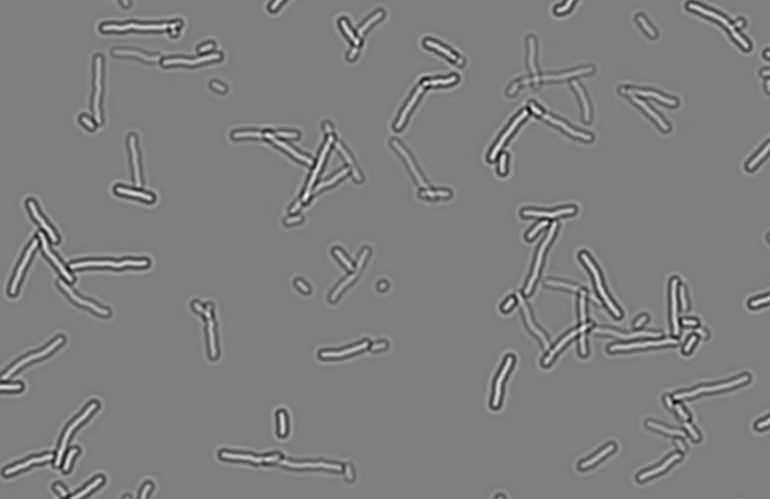
\includegraphics[width=0.65\textwidth]{frame.png}
      \caption{Sample image from our simulated microscope footage.}
      \label{fig:frame}
    \end{figure}

    The simulated videos and their associated metadata are passed into our neural network written in PyTorch. We used a CNN-TCN (Convolutional Neural Network, Temporal Convolutional Network) hybrid model. The CNN performs feature extraction on the each individual frame. It is implemented using the pretrained model ResNet50 which outputs 2048 spatial features for every input video. The TCN performs a temporal convolution on the input data and converts that to 64 temporal features. Finally, a fully connected layer takes the 64 temporal features and converts them to a single number. For every set of 5 frames window fed into the CNN-TCN, the model outputs one emergence index. By passing all possible 5 frame windows into the model in series, we can generate an emergence curve for every input video. Similarly, we can use thresholding to determine the onset time of the aggregation. A threshold of 1.5 appeared to produce the best results.

    To test the performance of our PyTorch model, we compared our results against a classical computer vision baseline. The classical computer vision pipeline first uses edge detection to identify individual particles. Next, it applies a closing operation to fill in each of the indicidual particles. It then identifies individual clusters as connected groups of white pixels. The computer vision model can then estimate the average size of the clusters by counting the number of white pixels in each connected group. This emergence index metric is not the same as that used in the digital twin simulator, where cluster size is computed in number of particles. In particular, it is vulnerable to differences in the size of particles. For this reason, we map all produced emergence curves onto the range $[0,1]$ before doing any performance comparisons.
  \end{block}
\end{column}

\separatorcolumn

\begin{column}{\colwidth}

  \begin{block}{Results}
    First and foremost, the machine learning model and computer vision models both produce reasonable emergence curves and onset estimates. In figure~\ref{fig:curve} below is a normalized comparison of curves produced by the digital twin and the two pipelines for a single simulated video.

    \begin{figure}[h]
      \centering
      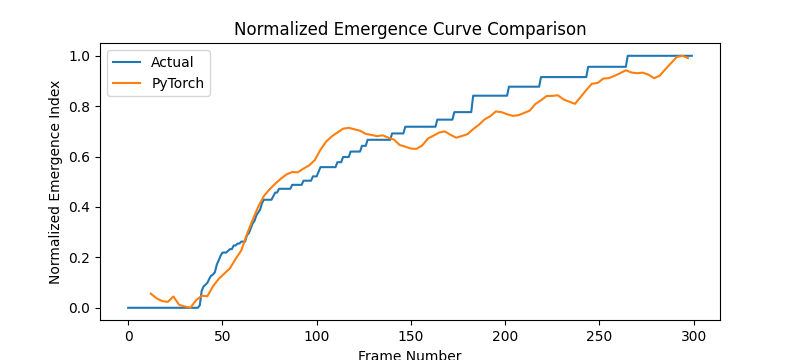
\includegraphics[width=0.75\textwidth]{result_norm.png}
      \caption{Normalized comparison of emergence curves from the digital twin and the two pipelines.}
      \label{fig:curve}
    \end{figure}

    The onset estimates produced by both pipelines were also quite accurate to that provided by the digital twin simulator. In figure~\ref{fig:onset} below is a comparison of onset estimate errors for the two pipelines.

    \begin{figure}[h]
      \centering
      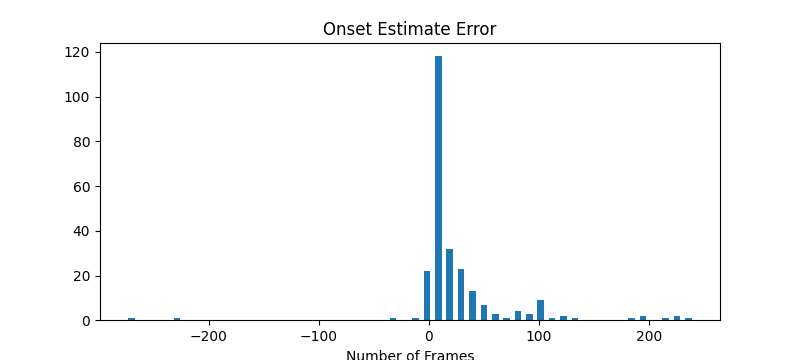
\includegraphics[width=0.75\textwidth]{result_onset_error.png}
      \caption{Onset estimate error distributions for the two pipelines.}
      \label{fig:onset}
    \end{figure}
   \end{block}

  \begin{block}{Conclusions}
    Both pipelines produced sensible emergence curves and reasonably accurate onset estimates. The machine learning model did not provide much improvement over the classical computer vision baseline in this particular test. This is not a failure of the machine learning model but rather a testament to the success of the computer vision baseline.

    This project did not make full use of the unique capabilities of machine learning models. Future work should make use of the generality of machine learning models. Testing the ability of machine learning models to infer physical parameters (e.g., determining particle aggregation probability directly from video) or to analyze more complicated physical phenomena could further emphasize the benefits that machine learning models can have.
  \end{block}

  \begin{block}{Acknowledgements and References}
    Special thanks to Professor Sang-Hyun Oh <sang@umn.edu> and to his graduate student <howey024@umn.edu> for their guidance throughout the semester.

    \nocite{*}
    \footnotesize{\bibliographystyle{plain}\bibliography{poster}}

  \end{block}

\end{column}

\separatorcolumn
\end{columns}
\end{frame}

\end{document}
